\documentclass[]{article}
\usepackage[margin=2.5cm]{geometry}
\usepackage{graphicx}

%opening
\title{Grundlagen der Startplanung}
\author{Ida Hönigmann}

\newenvironment{question}{\vspace{8mm}\noindent\bfseries}{\\}

\begin{document}

\maketitle

\section{Einführung in das Semesterprogramm}
\begin{question}
	Erläutern Sie wesentliche Faktoren, die die Entwicklung der Stadt beeinflussen. Gruppieren Sie diese.
\end{question}
TODO

\begin{question}
	''Stadtplanung ist eine Wissenschaft, eine Kunst, eine politische Bestrebung.'' Diskutieren Sie dies.
\end{question}
\begin{itemize}
	\item Wissenschaft: Kenntnisse der Stadtstruktur, Dienstleistungen und Beziehung der Bestandteile und Verkehrsbewegungen zu gewinnen;
	\item Kunst: Ziel der Bestimmung der Bodenordnung, Anordnung von Flächennutzungen und Verkehrswegen und Gebäudeentwurfes nach Grundsätzen, die Ordnung, Gesundheit und Wirtschaftlichkeit sichern;
	\item politische Bestrebung: um Grundsätzen Wirksamkeit zu verliehen.
\end{itemize}

\begin{question}
	Was verstehen Sie unter ''Ordnungsaufgaben'', was unter ''Gestaltungsaufgaben'' in der Stadtplanung?
\end{question}
\begin{itemize}
	\item Ordnungsaufgaben: Fragen des Flächenanspruchs und der wechselseitigen Zuordnung verschiedener Nutzungen
	\item Gestaltungsaufgaben: dreidimensionale Gestaltung des städtischen Raumes
\end{itemize}

\section{Wien - Geschichte, Gegenwart, Zukunftsperspektiven}
\begin{question}
	Erläutern Sie die zentralen Rahmen- und Ausgangsbedingungen zum STEP 2025 in Wien. Wie reagiert der STEP auf diese Herausforderungen?
\end{question}
TODO

\begin{question}
	Benennen Sie einige zentrale Phasen der Wiener Stadtentwicklung und richten Sie den Fokus dabei vor allem auf die Entwicklung ab Mitte des 19. Jahrhunderts!
\end{question}
Wien entwickelte sich auf dem Ort eines römischen Legionslagers zu einer immer bevölkerungsreicheren Stadt. Aus Verteidigungszwecken wurde ein Befestigungswall um die Stadt errichtet, was jedoch ab dem 19. Jahrhundert zu einem Platzmangel führt. Eines der entscheidenden Projekte für die Stadt Wien ist daher der Umbau der Verteidigungsmauern zur Ringstraße.

Ein weiteres großes Projekt war die Regulierung der Donau. Vor und im 19. Jahrhundert kam es immer wieder zu Überschwemmungen, weswegen immer mehr Arme der Donau abgesperrt wurden. Nach dem Hochwasser im Jahr 1954 war klar, dass zusätzlich ein Entlastungsgerinne notwendig war. Der Bau dieses Neuen Donau ließ die sogenannte Donauinsel entstehen.

Im Zuge von Stadterweiterungen wird Anfang des 20. Jahrhunderts ist immer wieder vom kreisförmigen Stadtbild und dem grünen Ring um Wien die rede.

Viele Wiener lebten um 1900 in schlechten Wohnbedingungen. Um die Wohnungsnot zu bekämpfen werden in der Zeit des roten Wiens Wohnungsbauten von der Gemeinde Wien gebaut. Diese Wohnungen entsprechen wesentlich besseren Standards als davor in Wien üblich. Es wird begonnen Richtlinien und Bestimmungen in Form von Bauordnungen zu verordnen.

Nach dem zweiten Weltkrieg entstanden durch den steigenden Mobilisierungsgrad ermöglicht viele Entwicklungen an den Rändern der Stadt Wien. Es wurde Auto-freundlich gebaut und umgebaut. Allerdings wurde diese Entwicklung auch kritisch gesehen. So wird der Fokus der Stadtentwicklung in Wien auf die Erhaltung und Erneuerung gelegt.

Nach dem Fall der eisernen Mauer rückt Wien weiter ins Zentrum Europas. Es kommt immer wieder Überlegungen über eine Kooperation mit Bratislava.

\begin{question}
	Worin begründen sich die besonderen Herausforderungen der Wiener Stadtentwicklung?
\end{question}
Herausforderung: Strategien und Instrumente der Stadtentwicklung weiterzuentwickeln sodass Qualitätsstandards erhalten und neue, zukunftsgerichtete Qualitäten ermöglichen;

\begin{itemize}
	\item standortwirtschaftliche und infrastrukturelle Rahmenbedingungen für Investor*innen und Entwickler*innen sodass rasch, elastisch und innovativ auf Veränderungen reagiert werden kann und den Interessen und Bedürfnissen der Bevölkerung entsprochen wird;
	\item gebaute, (frei-)räumliche und ökologische Substanz der Stadt fit zu machen für Wachstum, Erhalten, Erneuern, Transformieren.;
	\item stabiles soziales Gleichgewicht; Diversität und Gleichstellung;
	\item kollektive Verantwortung und Kooperationsaufgabe von Politik, Wirtschaft und Bevölkerung;
	\item Prozesse von Planung, Managements, Umsetzung partizipativ und effizient gestalten.
\end{itemize}

\begin{question}
	Erläutern Sie wesentliche im STEP 2025 dokumentierte Prinzipien der Wiener Stadtentwicklung!
\end{question}
Aufbruch durch Wachstum und Entwicklungsdynamik kommt der ganzen Stadt zugute. lebenswerte Stadt bleiben (leben, arbeiten, lernen, austauschen). attraktives Wien für alle erlebbar sein.
Wettbewerbsfähigkeit und Unternehmergeist, Leistbarkeit, soziale Gerechtigkeit, Integration, ressourcenschonende Klima- und Umweltschutzpolitik alles gleich gewichtet.

STEP berücksichtigt Besonderheiten, Stärken und Schwächen des Standorts Wien.
STEP bezieht Fachkonzepten mit ein.
STEP ist für die Wiener Stadtentwicklung handlungsleitend.

\begin{question}
	Erläutern Sie die wesentlichen Ziele der vier Handlungsbereiche des STEP 2025!
\end{question}
\begin{itemize}
	\item Wir leisten uns Stadt
	
	\item Wien baut auf
	
	Qualitätsvolle Stadtstruktur und vielfältige Urbanität
	
	\item Wien wächst über sich hinaus
	
	Wachstum und Wissensgesellschaft transformieren die Metropolregion
	
	\item Wien ist vernetzt
	
	Weitsichtig, robust und tragfähig für Generationen
\end{itemize}

\begin{question}
	Diskutieren Sie den im STEP 2025 zum Ausdruck gebrachten Anspruch ''Wir leisten uns Stadt!'' (S. 12ff)
\end{question}
TODO

\begin{question}
	Diskutieren Sie den Anspruch des STEP 2025 an eine qualitätsvolle Stadtstruktur und vielfältige Urbanität! Benennen Sie die zentralen Ziele! (S. 34)
\end{question}
TODO

\begin{question}
	Was sind die im STEP 2025 dokumentierten Aspekte der Flächensicherung für das Stadtwachstum? (S. 48ff)
\end{question}
TODO

\begin{question}
	Was versteht der STEP 2025 unter einer ''ausgewogenen, polyzertrischen Standortentwicklung''? (S. 64)
\end{question}
TODO

\begin{question}
	Diskutieren Sie das Leitbild zur Siedlungsentwicklung! (S. 67)
\end{question}
TODO

\begin{question}
	Diskutieren Sie den Anspruch and die Entwicklung der Metropolregion! (S. 88ff)
\end{question}
TODO

\begin{question}
	Was sind Fachkonzepte zum STEP25?
\end{question}
Begleitende Dokumente zum STEP die spezifische Information und Herausforderungen und Lösungsansätze zu verschiedensten Spezialgebieten der Stadtentwicklung enthalten. z.B. Produktive Stadt, Mittelpunkt des Städtischen Lebens, Grün- und Freiraum, Öffentlicher Raum, Mobilität, Hochhäuser, Partizipative Stadtentwicklung, Masterplan Gründerzeit

\begin{question}
	Welche Wirkungen entfalten STEP 2025 und die Fachkonzepte zum STEP?
\end{question}
TODO

\begin{question}
	Welchen Stellenwert besitzt die Smart City Rahmenstrategie der Stadt Wien?
\end{question}
langfristige Dachstrategie, Zielhorizont 2050

\begin{question}
	Erläutern Sie die drei Handlungsfelder auf die sich die Smart City Rahmenstrategie der Stadt Wien bezieht!
\end{question}
\begin{itemize}
	\item Ressourcen (Energie, Mobilität, Infrastruktur, Gebäude)
	\item Lebensqualität (Soziale Inklusion, Partizipation, Gesundheit, Umwelt)
	\item Innovation (Bildung, Wirtschaft, Forschung, Technologie)
\end{itemize}

\section{Theorie und Methodik der Stadtplanung}
\begin{question}
	Erläutern Sie die wesentlichen Grundfunktionen der räumlichen Planung!
\end{question}

\begin{itemize}
	\item Vernetzung unterschiedlicher Interessen
	\item Zukunftsperspektive
	\item Abbau von Konflikten zwischen Raumansprüchen
	\item Verteilung der Nutzungen und Gestaltung der Raumansprüche
	\item Verhindern vermeidbarer Unterschiede der Lebensbedingungen
	\item Erhaltung natürliche und kulturelle Elemente
	\item Schonung naturgebundener Ressourcen
\end{itemize}


\begin{question}
	Woran orientiert sich die Planung? Stellen Sie das Wirkgeflecht grafisch dar!
\end{question}

\begin{itemize}
	\item Rechtsvorgaben
	\item politische Zielsetzungen
	\item politische Programme und Richtlinien
	\item Erkenntnisse aus Wissenschaft und Praxis
	\item Referenzprojekte und historische Vorbilder
	\item Zielsetzungen und Qualitätsansprüche aus Bevölkerung
	\item eigene Erfahrungen, Werthaltungen und Prinzipien
\end{itemize}

insgesamt eine Mischung aus

\begin{itemize}
	\item allgemein und speziell,
	\item verbindlich und unverbindlich,
	\item normativ und deskriptiv,
	\item kurzfristig und langfristig
	\item Vorschriften, Zielsetzungen, Wertsetzungen und Handlungsprinzipien
\end{itemize}

\begin{figure}[h!]
	\centering
	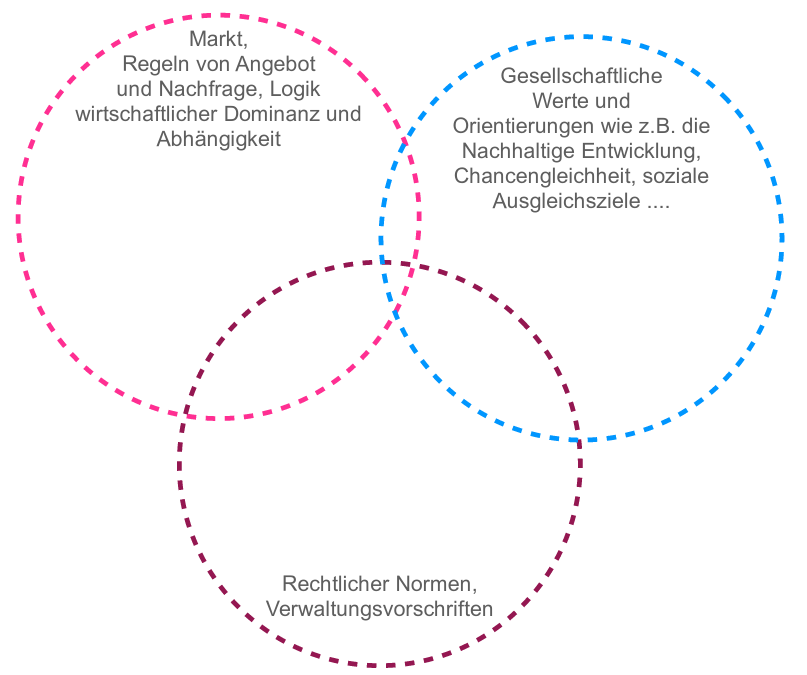
\includegraphics[width=0.5\linewidth]{images/planung_wirkgeflecht}
	\label{fig:planungwirkgeflecht}
\end{figure}


\begin{question}
	Diskutieren Sie das Verhältnis von Planung, Politik und Verwaltung!
\end{question}
\begin{itemize}
	\item Planung: Entscheidungsvorbereitung
	\item Politik: Entscheidung über Alternativen
	\item Verwaltung: Administrativer Vollzug
\end{itemize}

In Praxis: Vermischung der Ebenen z.B. bereits Auswahl von nur wenigen Alternativen in Planungsphase oder Politik gibt Rahmenbedingungen zur Planung vor.


\begin{question}
	Wer entwickelt die Stadt? Welche Aufgabe nimmt die Stadtplanung in dem Akteursgeflecht ein?
\end{question}
\begin{itemize}
	\item Planungsträger - Auftraggeber der Planung z.B. Gemeinde
	\item Planer - Bearbeitung der Pläne unter fachlichen Aspekten z.B. Stadtplanungsamt
	\item Entscheider - Entscheiden über Entwürfe z.B. Gemeinderat
	\item Durchführender - Durchführen von Maßnahmen z.B. Bauträger
	\item Beteiligte/Betroffene - Personen und Institutionen die von den Maßnahmen berührt werden z.B. Anwohner, Investoren
\end{itemize}


\begin{question}
	Was müssen Pläne leisten? Welche Anforderungen sind mit dem Plan verknüpft?
\end{question}
\begin{itemize}
	\item Orientierung, Rechtssicherheit
	\item Inhalte bildlich vermitteln, Argumentationen abbilden, Dialoge anregen
\end{itemize}

Anforderungen:
\begin{itemize}
	\item Vermittlung / Kommunikation
	\item Steuerungsintention
	\item Überschaubare und kontrollierbare Ziel-Mittel-Verknüpfung
	\item Festlegung von Prioritäten und Präferenzen
	\item Zeitlich festgelegte Verwirklichungsstufen
	\item Grafische Darstellung
\end{itemize}


\begin{question}
	In der Planungspraxis wird zwischen einer langfristig orientierten Querschnittplanung und einer projekt- bzw. aufgabenspezifischen Planung unterschieden. Erläutern Sie dies.
\end{question}
\begin{itemize}
	\item Langfristig orientierte Querschnittsplanung:
	
	z.B. Stadtentwicklungskonzept
	
	\begin{itemize}
		\item Darstellung von Zielen, Prioritäten, Alternativen, Perspektiven
		\item langfristige Orientierung
		\item Stadt- bzw. Gemeindegebiet
		\item Maßstab: 1:25.000 bis 1:10.000
		\item Schwerpunktsetzend
		\item flexibel/variabel
		\item präventiv/perspektivisch
		\item informell
	\end{itemize}

	\item Projekt- bzw. Aufgabenbezogene Planung:
	
	z.B. Gestaltungsentwurf
	
	\begin{itemize}
		\item Auf kurzfristige Umsetzung angelegt
		\item Maßstab: 1:500 bis 1:200
		\item Präzise
		\item Umsetzungsbezogen
	\end{itemize}
\end{itemize}


\begin{question}
	Erläutern Sie wesentliche Herausforderungen der Innenstadtentwicklung!
\end{question}
TODO


\begin{question}
	Auf welchen Steuerungsformen basiert die Raumplanung?
\end{question}
TODO


\begin{question}
	Diskutieren Sie wesentliche Unterscheidungsmerkmale zwischen der Objektplanung und der Stadtplanung / örtlichen Raumplanung!
\end{question}
siehe Grafik \ref{fig:vergleichstaedtebauobjektplanung}
\begin{figure}[h!]
	\centering
	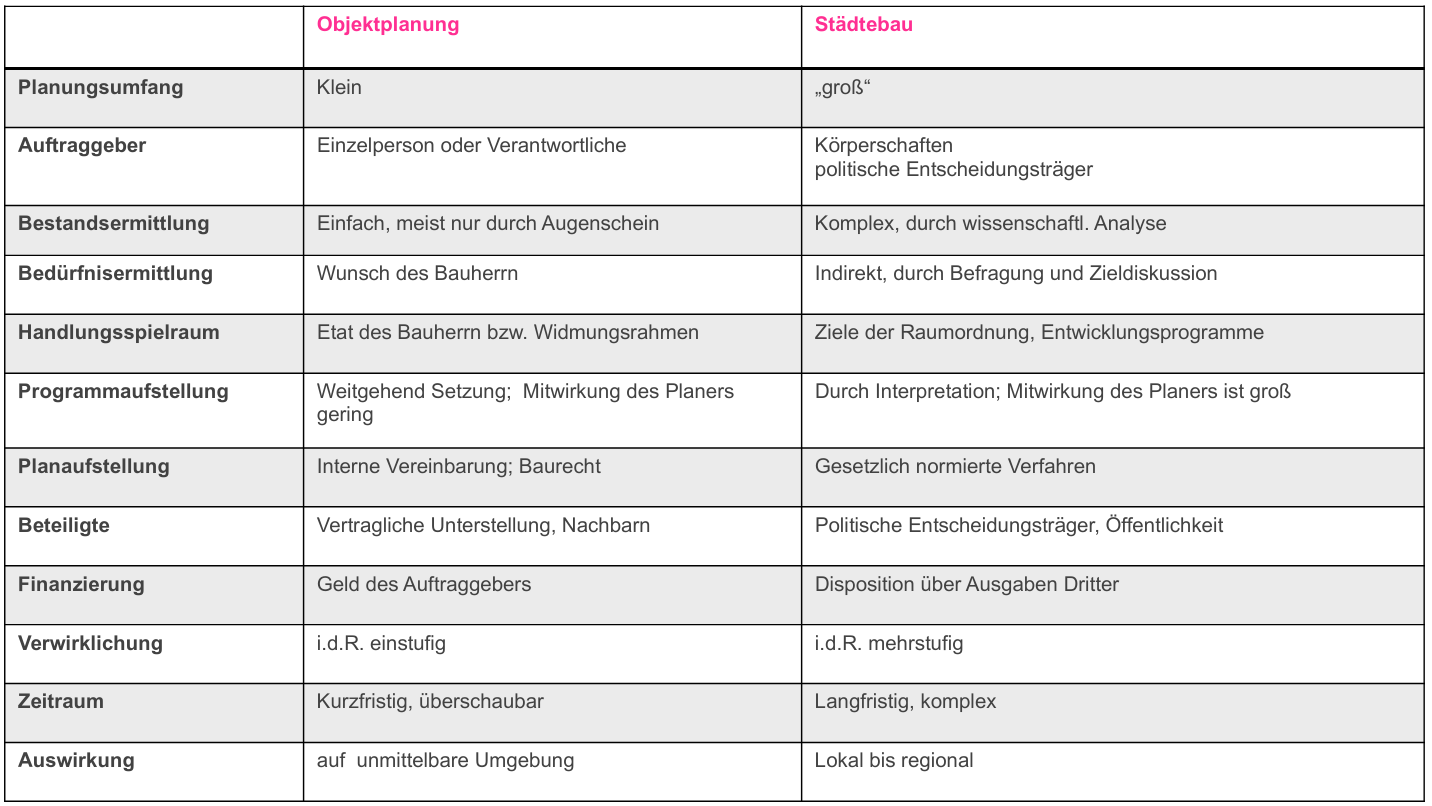
\includegraphics[width=0.7\linewidth]{images/vergleich_staedtebau_objektplanung}
	\caption{Tabellarischer Vergleich}
	\label{fig:vergleichstaedtebauobjektplanung}
\end{figure}


\begin{question}
	Jeder Entwurfsprozess folgt einer wissenschaftlichen Methodik. Nehmen Sie dazu Stellung und stellen Sie die Entwurfsmethodik in den einzelnen Schritten dar (Diagramm, Erläuterungen)!
\end{question}
TODO


\begin{question}
	Welche Informationsebenen umfasst die Bestandsanalyse?
\end{question}
TODO


\begin{question}
	Benennen Sie einige Techniken der Bestandsaufnahme in der Stadtplanung!
\end{question}
TODO


\section{Instrumente der Örtlichen Raumplanung}
\begin{question}
	Was ist unter dem Begriff ''ÖROK'' zu verstehen? Welche Aufgaben kommen der ÖROK zu?
\end{question}
Österreichische Raumordnungskonferenz

wurde zur besseren Abstimmung als politisches Organ gegründet.


\begin{question}
	Welche Kompetenzen in raumplanerischen Fragen hat die ÖROK?
\end{question}
TODO


\begin{question}
	Erläutern Sie wichtige Zielsetzungen und Ansprüche des ÖREK 2030!
\end{question}
TODO


\begin{question}
	Im ÖREK 2030 sind einige Megatrens benannt. Welche sind dies?
\end{question}
TODO


\begin{question}
	Was verbirgt sich in dem 10-Punkte-Programm des ÖREK 2030?
\end{question}
TODO


\begin{question}
	Welche Raumtypen werden im ÖREK 2030 definiert?
\end{question}
TODO


\begin{question}
	Benennen Sie einige exemplarische Herausforderungen in den einzelnen Raumtypen!
\end{question}
TODO


\section{Instrumente der Stadtplanung}
\begin{question}
	Erläutern Sie die unterschiedlichen Typen von Plänen (nach Albers)!
\end{question}
TODO


\begin{question}
	Erläutern Sie die Unterschiede zwischen formellen und informellen Instrumente! Benennen Sie Beispiele!
\end{question}
TODO


\begin{question}
	Erläutern Sie die wesentlichen Instrumente der Raumplanung auf der örtlichen Ebene!
\end{question}
TODO


\begin{question}
	Ordnen Sie Plandarstellungen den Instrumenten zu!
\end{question}
TODO


\section{Instrumente auf der Örtlichen Ebene}
\begin{question}
	Was verstehen Sie unter einem Örtlichen Raumordungsprogramm in NÖ? Was sind seine Bestandteile?
\end{question}
TODO

\begin{question}
	Erläutern Sie grundlegende Ansprüche an das Örtliche Entwicklungskonzept!
\end{question}
TODO

\begin{question}
	Was verstehen Sie unter einem ''geregelten Verfahren'' in der Planung? Weshalb ist dies notwendig?
\end{question}
TODO


\begin{question}
	''Vom Reagieren zum Agieren'' - Erläutern Sie die Relevanz bezogen auf das ÖEK!
\end{question}
TODO

\begin{question}
	Welche Rechte entfaltet eine ÖEK, ein Flächenwidmungsplan, ein Bebauungsplan?
\end{question}
TODO

\begin{question}
	Was unterscheidet den Flächenwidmungsplan vom Bebauungsplan? Erläutern Sie die entsprechende Widmungskategorien und Wirkungen!
\end{question}
TODO

\begin{question}
	Was sind die Mindestinhalte eines Bebauungsplanes?
\end{question}
TODO

\begin{question}
	Erläutern Sie die wesentlichen Unterschiede zwischen einem Örtlichen Entwicklungskonzept und einem Flächenwidmungsplan bezogen auf den ''Rechtlichen Charakter'', die ''Aufgaben'' und die ''Inhalte''!
\end{question}
TODO

\begin{question}
	Wie definiert die Wiener Bauordnung die Anforderungen an Flächenwidmungs- und Bebauungspläne?
\end{question}
TODO

\begin{question}
	Erläutern Sie die in der Bauordnung festgelegten Widmungsarten!
\end{question}
TODO

\begin{question}
	Was unterscheidet den Bebauungsplan vom Flächenwidmungsplan?
\end{question}
TODO

\begin{question}
	Was verstehen Sie unter ''Bauklasseneinteilung'' oder ''Bauweise''?
\end{question}
TODO


\end{document}
